\documentclass[11pt,a4paper]{article}
\usepackage[margin=21mm,headheight=15pt]{geometry}
\usepackage{cmap}
\usepackage[LGR,T1]{fontenc}
\usepackage[utf8]{inputenc}
\usepackage[greek,english]{babel}
\usepackage{alphabeta,lmodern,newunicodechar}
\usepackage{amsmath,amssymb,booktabs,array,tabularx,tikz,xcolor,hyperref,fancyhdr}
\usetikzlibrary{arrows.meta,positioning}
\definecolor{ink}{HTML}{174D67}\definecolor{soft}{HTML}{EDF5F7}
\hypersetup{unicode=true,colorlinks=true,linkcolor=ink,urlcolor=ink,pdftitle={Από τα pods στην κβαντική πολιτική},pdfauthor={QRL-Lab — Codex}}
\pagestyle{fancy}\fancyhf{}\fancyhead[L]{\small\sffamily QRL-Lab · Οδηγός κατανόησης}\fancyfoot[R]{\thepage}
\setlength{\emergencystretch}{3em}
\setlength{\parindent}{0pt}\setlength{\parskip}{7pt}\linespread{1.08}
\newcommand{\page}[2]{\clearpage\pdfbookmark[0]{#1}{topic\thepage}{\sffamily\color{ink}\LARGE #1\par}\vspace{3pt}{\sffamily\large #2\par}\vspace{8pt}}
\newcommand{\idea}[1]{\par\noindent\colorbox{soft}{\parbox{\dimexpr\linewidth-2\fboxsep}{\textbf{Κράτησε αυτό:} #1}}\par}
\newcommand{\think}[1]{\par\textbf{Στάση για σκέψη.} #1}
\newcommand{\src}[1]{\vfill{\footnotesize\color{ink}\textbf{Πηγή / έλεγχος:} #1\par}}
\newcommand{\code}[1]{{\footnotesize\nolinkurl{#1}}}
\newcommand{\ket}[1]{\lvert #1\rangle}
\begin{document}
{\sffamily\color{ink}\LARGE Από τα pods στην κβαντική πολιτική\par}
{\sffamily Σύντομος οδηγός κατανόησης · 29/10/2026 · προσχέδιο 1}\par
Πώς αποφασίζουμε πότε να προσθέσουμε pods στο Redis; Πρώτα η διαίσθηση, μετά οι εξισώσεις. Δεν χρειάζεται προγραμματισμός. Τα «διδακτικά» αριθμητικά παραδείγματα είναι υποθετικά, όχι αποτελέσματα πειραμάτων.

{\sffamily\color{ink}\Large 1 · Ένας ελεγκτής, ένας κόσμος\par}
Ας κρατήσουμε σε όλο τον οδηγό το ίδιο σύστημα: αιτήματα φτάνουν στο Redis, τα ενεργά pods τα εξυπηρετούν και όσα περιμένουν σχηματίζουν ουρά.

\begin{center}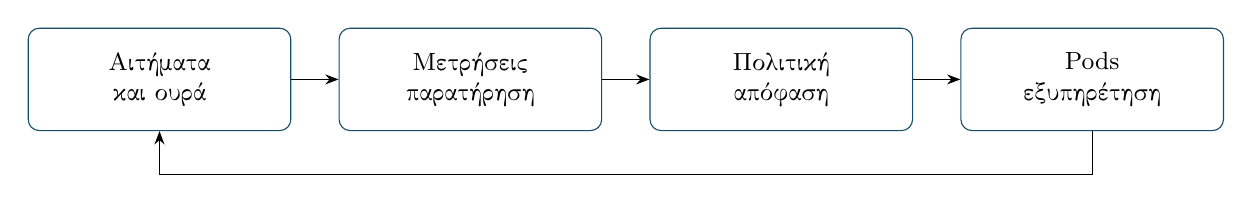
\begin{tikzpicture}[node distance=6mm,box/.style={draw=ink,rounded corners,align=center,font=\small,minimum height=13mm,text width=31mm},>=Stealth]
\node[box] (w) {Αιτήματα\\και ουρά};
\node[box,right=of w] (o) {Μετρήσεις\\παρατήρηση};
\node[box,right=of o] (p) {Πολιτική\\απόφαση};
\node[box,right=of p] (a) {Pods\\εξυπηρέτηση};
\draw[->] (w)--(o);\draw[->] (o)--(p);\draw[->] (p)--(a);
\draw[->] (a.south) -- ++(0,-.55) -| (w.south);
\end{tikzpicture}\end{center}

Ένα επεισόδιο είναι μια διαδρομή μέχρι το τέλος της· reset είναι η επανεκκίνηση από αρχική κατάσταση. Σε κάθε χρονικό βήμα (tick) ο ελεγκτής βλέπει επτά χαρακτηριστικά: πλήθος αφίξεων, δυναμικότητα, CPU, μνήμη, p95 καθυστέρηση, ενεργά pods και pods που περιμένουν να ξεκινήσουν. Το p95 είναι το όριο κάτω από το οποίο βρίσκεται περίπου το 95\% των τιμών καθυστέρησης.

Η ενέργεια $a_t$ είναι \textbf{μείωση, αναμονή ή αύξηση}. Ο δείκτης $t$ σημαίνει «τώρα». Το νέο pod δεν βοηθά αμέσως: η προεπιλεγμένη καθυστέρηση εκκίνησης είναι πέντε ticks. Η μείωση ακυρώνει πρώτα το πιο πρόσφατο εκκρεμές pod.

Η παρατήρηση δεν αποκαλύπτει πλήρως την πραγματική ουρά. Γι' αυτό το ιστορικό μπορεί να βοηθήσει: η ίδια CPU τώρα μπορεί να ανήκει είτε σε ανερχόμενο είτε σε υποχωρούν φορτίο.

\think{Αν περιμένουμε να γεμίσει η ουρά πριν ζητήσουμε pod, ποιο χρονικό κόστος αγνοούμε; Απάντηση στη σ. 19. Διαδρομή: κλασικά μοντέλα σ. 5–11, αξιολόγηση σ. 12–13, κβαντικά σ. 14–18.}
\src{\code{poisson_ms.py}: \code{FEATURES}, \code{Params.delay}, \code{PoissonMSEnv._apply}. Όλα τα σύντομα ονόματα κώδικα αναφέρονται στο \code{code-poisson/tuning/}. Το tick είναι μονάδα προσομοίωσης, όχι μετρημένο δευτερόλεπτο πραγματικού cluster.}

\page{2 · Το φορτίο δεν είναι ρολόι}{Γιατί Poisson και γιατί εκθετικά διαστήματα;}
«Ρυθμός $\lambda$» σημαίνει πόσα αιτήματα περιμένουμε ανά μονάδα χρόνου, όχι πόσα θα έρθουν υποχρεωτικά. Με σταθερό ρυθμό και ανεξάρτητες αφίξεις:
\[
 N\sim\operatorname{Poisson}(\lambda\Delta),\qquad
 \Pr(N=k)=e^{-\lambda\Delta}\frac{(\lambda\Delta)^k}{k!}.
\]
Το $N$ μετρά αιτήματα σε διάστημα μήκους $\Delta$, το $k$ είναι ένα πιθανό πλήθος και το $k!$ είναι το γινόμενο των θετικών ακεραίων μέχρι το $k$.

\textbf{Διδακτικό παράδειγμα.} Για $\lambda=2$ αιτήματα ανά tick και $\Delta=1$, η πιθανότητα να μη φτάσει κανένα είναι $e^{-2}\approx0.135$. Άρα «μέσος ρυθμός δύο» δεν σημαίνει «ένα αίτημα κάθε μισό tick».

Στην ομογενή διαδικασία Poisson το διάστημα $T$ ανάμεσα σε διαδοχικές αφίξεις είναι εκθετικό:
\[
 \Pr(T>u)=e^{-\lambda u},\qquad \mathbb{E}[T]=1/\lambda.
\]
Το $u$ είναι χρόνος αναμονής και $\mathbb{E}$ σημαίνει μέση αναμενόμενη τιμή. Η εκθετική κατανομή περιγράφει \emph{χρόνους}, ενώ η Poisson \emph{πλήθη}. Η χρήση Poisson για τους ίδιους τους χρόνους αναμονής δεν δημιουργεί σωστή διαδικασία Poisson.

Ο κώδικάς μας χρησιμοποιεί ισοδύναμη κατασκευή μέσα σε κάθε tick: τραβά πλήθος Poisson, τοποθετεί τόσους ομοιόμορφους χρόνους μέσα στο tick και τους ταξινομεί. Ο ρυθμός παραμένει σταθερός μέσα στο tick.

\idea{Τυχαίος χρόνος άφιξης και τυχαίο πλήθος συνδέονται, αλλά δεν είναι το ίδιο μέγεθος.}
\src{\code{poisson_ms.py}: \code{Workload.next_tick}. Θεωρία: ProbabilityCourse, §11.1.2 [Π1, σ. 20]. Ο αριθμητικός υπολογισμός παραπάνω προκύπτει από την εξίσωση, όχι από run.}

\page{3 · Όταν αλλάζει ο ρυθμός}{Ημέρα, εκρήξεις και επίμονος θόρυβος}
Ένα σύστημα έχει ώρες αιχμής και απότομα κύματα. Αν ο ρυθμός $\lambda(t)$ είναι δεδομένη μεταβαλλόμενη συνάρτηση, έχουμε μη ομογενή διαδικασία Poisson (NHPP):
\[
 N_{[a,b]}\sim\operatorname{Poisson}\!\left(\int_a^b\lambda(u)\,du\right).
\]
Το ολοκλήρωμα είναι ο συνολικός αναμενόμενος αριθμός αιτημάτων στο διάστημα. Με μεταβαλλόμενο ρυθμό, τα διαστήματα δεν είναι γενικά ανεξάρτητα εκθετικά με μία κοινή παράμετρο.

Στο περιβάλλον μας ο ρυθμός ανά tick είναι:
\[
 \lambda_t=b\,[1+A\sin(2\pi t/P+\varphi)]\,B_t\,e^{x_t}.
\]
Το $b$ είναι βάση, $A$ εύρος περιοδικής μεταβολής, $P$ περίοδος και $\varphi$ αρχική φάση (διαφορετική από το $\phi$ παρακάτω). Το $B_t$ επιλέγει ήρεμη κατάσταση ή έκρηξη. Το $e^{x_t}$ κρατά θετικό τον πολλαπλασιαστικό θόρυβο.
\[
 x_t=\phi x_{t-1}+\sqrt{1-\phi^2}\,\sigma\epsilon_t,
 \qquad \epsilon_t\sim\mathcal N(0,1).
\]
Εδώ $\phi$ ελέγχει πόσο επιμένει ο προηγούμενος θόρυβος, $\sigma$ το μέγεθός του και $\epsilon_t$ μια νέα τυχαία διαταραχή.

\idea{Μια έκρηξη επιμένει για διαδοχικά ticks· ο ελεγκτής αντιμετωπίζει διαδοχικές δύσκολες στιγμές, όχι ανεξάρτητες μεμονωμένες αιχμές.}
\textbf{Ονομασίες, αν θέλεις περισσότερη ακρίβεια.} Η αλλαγή ήρεμου/έντονου καθεστώτος είναι αλυσίδα Markov: η επόμενη κατάσταση εξαρτάται από την τωρινή. Ο κώδικας αλλάζει μόνο στα όρια ticks, άρα πρόκειται για διακριτό ανάλογο MMPP δύο καταστάσεων. Με τυχαίο ρυθμό συνολικά έχουμε διαδικασία Cox· υπό δεδομένη διαδρομή ρυθμού, NHPP.

\think{Αν μοιραστούν δύο μοντέλα την ίδια διαδρομή αφίξεων, ποια πηγή αδικίας αφαιρούμε;}
\src{\code{poisson_ms.py}: \code{Workload.rate}, \code{Workload.next_tick}. NHPP: [Π2, σ. 20]. Η ονομασία MMPP είναι συντομογραφία σχεδίασης, όχι ισχυρισμός υλοποίησης συνεχούς MMPP.}

\page{4 · Τι ανταμείβουμε;}{Από την ουρά σε έναν στόχο μάθησης}
Η δυναμικότητα είναι $C_t=\mu n_t$: κάθε ενεργό pod προσφέρει ρυθμό $\mu$ και έχουμε $n_t$ ενεργά pods. Το εκκρεμές pod χρεώνεται, αλλά ακόμη δεν εξυπηρετεί.

Με $W$ μονάδες εργασίας ήδη στην ουρά, η προσεγγιστική καθυστέρηση ενός νέου αιτήματος είναι:
\[
 \ell\approx\ell_0+\frac{W+1}{C_t}.
\]
Το $\ell_0$ είναι βασική καθυστέρηση. Αυτή είναι \textbf{εκτίμηση κατά την είσοδο}, με την τωρινή δυναμικότητα· δεν αναθεωρείται όταν αλλάξουν αργότερα τα pods. Δεν είναι μέτρηση πραγματικής απόκρισης Redis.

Η ανταμοιβή (reward) ανά tick είναι:
\[
 r_t=S_t-c_p(n_t+p_t)-w_s I_t-w_d D_t.
\]
$S_t$: εργασία που εξυπηρετήθηκε. $p_t$: εκκρεμή pods. $c_p$: κόστος ανά pod. $I_t$: ένδειξη παραβίασης στόχου υπηρεσίας (SLO). $D_t$: απορριφθέν έργο. Τα $w_s,w_d$ ορίζουν πόσο βαριά τιμωρούμε αυτές τις αστοχίες.

\textbf{Διδακτικό στιγμιότυπο με τα βάρη του κώδικα:} αν εξυπηρετήθηκαν $60$ αιτήματα, υπάρχουν $6$ ενεργά pods, κανένα εκκρεμές, καμία παραβίαση και καμία απόρριψη, τότε $r=60-3\cdot6=42$. Το $3$ είναι το προεπιλεγμένο $c_p$· το στιγμιότυπο είναι υποθετικό.

Παραβίαση μετρά όταν το p95 ξεπερνά το SLO ή υπάρχουν απορρίψεις. Στο τέλος του επεισοδίου χρεώνεται επίσης η ανολοκλήρωτη ουρά ως απορριφθέν έργο και ενεργοποιεί παραβίαση. Δεν κρύβουμε δουλειά στο reset.

Στην εκπαίδευση του παρόντος συμβολαίου αποθηκεύουμε $r_t/10$ και κανονικοποιημένες παρατηρήσεις· τα αποτελέσματα αξιολόγησης κρατούν την αρχική κλίμακα reward. Η κλίμακα δεν αλλάζει τον επιθυμητό συμβιβασμό, αλλά αλλάζει το μέγεθος των ενημερώσεων.

\idea{Η ανταμοιβή ορίζει τον συμβιβασμό μας. Μεγάλη ανταμοιβή δεν αρκεί χωρίς SLO, κόστος, απορρίψεις και αλλαγές pods.}
\src{\code{poisson_ms.py}: \code{Params}, \code{serve_tick}, \code{PoissonMSEnv.step}. Η ουρά είναι μοντέλο ρευστής εργασίας FIFO, όχι πλήρης προσομοίωση Redis. Κλίμακες μάθησης: \code{pms_adapter.py}, \code{.lab/j64/final.json}. Στον παλιό simulator η latency δεν εξαρτιόταν από pods (PLAN F1)· δεν χρησιμοποιείται ως απόδειξη πραγματικής υπεροχής.}

\page{5 · Μάθηση από συνέπειες}{Τι μαθαίνει το Q και τι αλλάζει η εκπαίδευση;}
Στην ενισχυτική μάθηση (reinforcement learning, RL), δεν δίνουμε στον ελεγκτή τη σωστή ενέργεια για κάθε στιγμή. Του δίνουμε ανταμοιβές από τις συνέπειες των ενεργειών του.

Η πολιτική (policy) είναι ο κανόνας επιλογής ενέργειας. Μια συνάρτηση αξίας ενέργειας $Q(s,a)$ εκτιμά πόσο καλή θα είναι μια ενέργεια $a$ στην παρατήρηση/ιστορικό $s$, μαζί με τη συνέχεια:
\[
 Q(s,a)\approx\mathbb E\!\left[r_t+\gamma r_{t+1}+\gamma^2r_{t+2}+\cdots\right].
\]
Το $\gamma$ είναι συντελεστής προεξόφλησης: όσο μικραίνει, τόσο λιγότερο μετρά η μακρινή συνέχεια. Το $Q$ δεν είναι πιθανότητα ούτε μόνο πρόβλεψη του επόμενου φορτίου.

Ένα βαθύ Q-δίκτυο (DQN) υπολογίζει αυτές τις αξίες με νευρωνικό δίκτυο. Οι παράμετροι είναι οι ρυθμιζόμενοι αριθμοί του. Η εκπαίδευση αλλάζει παραμέτρους για να φέρνει προβλέψεις κοντά σε στόχους που προκύπτουν από εμπειρίες.

Κρατάμε εμπειρίες $(s,a,r,s',d)$ σε μνήμη επανάληψης (replay buffer): τι είδαμε, τι κάναμε, τι πήραμε, τι ακολούθησε και αν τελείωσε το επεισόδιο ($d$). Η επανάληψη παλιών εμπειριών μειώνει την εξάρτηση μόνο από τις πιο πρόσφατες στιγμές.

Στην εκπαίδευση η $\epsilon$-greedy επιλογή δοκιμάζει τυχαία ενέργεια με πιθανότητα $\epsilon$. Στην αξιολόγησή μας επιλέγουμε την καλύτερη εκτιμώμενη ενέργεια χωρίς μάθηση. Η λειτουργία μετά την εκπαίδευση ονομάζεται inference.

\think{Γιατί μια προσωρινά ακριβή αύξηση pods μπορεί να έχει καλύτερο $Q$ από την αναμονή;}
\src{\code{legacy/agent_lstm_fixed.py}: \code{act}, \code{remember}, \code{replay}. Εισαγωγή Double DQN: [Μ1, σ. 20].}

\page{6 · Double DQN και τρία βήματα}{Πώς φτιάχνεται ο στόχος μιας διόρθωσης;}
Χρησιμοποιούμε ένα δίκτυο online, με παραμέτρους $\theta$, που μαθαίνει συνεχώς, και ένα target, με παραμέτρους $\bar\theta$, που αντιγράφεται περιοδικά. Ο πιο αργός στόχος δίνει σταθερότερο σημείο αναφοράς.

Στο απλό DQN ο στόχος είναι $r+\gamma\max_a Q_{\bar\theta}(s',a)$. Στο Double DQN χωρίζουμε επιλογή και αποτίμηση:
\[
 a^*=\arg\max_a Q_\theta(s',a),\qquad
 y=r+\gamma(1-d)Q_{\bar\theta}(s',a^*).
\]
Το $\arg\max$ επιστρέφει την ενέργεια με τη μεγαλύτερη αξία. Το $d=1$ σημαίνει πραγματικό τέλος, οπότε δεν υπάρχει μελλοντικός όρος. Ο στόχος $y$ θεωρείται σταθερός κατά τη διόρθωση των βαρών (χωρίς gradient). Gradient είναι η ευαισθησία του σφάλματος σε κάθε βάρος.

\textbf{Διδακτικό παράδειγμα.} Online αξίες για μείωση/αναμονή/αύξηση: $(4,5,3)$, target αξίες: $(6,2,1)$. Το online επιλέγει αναμονή και το target την αποτιμά σε $2$. Με $r=1$, $\gamma=0.9$ και χωρίς τέλος, $y=2.8$. Το DQN θα χρησιμοποιούσε το $6$ και θα έδινε $6.4$. Αυτό δείχνει τη διαφορά υπολογισμού, όχι ότι κάθε Double DQN εκτίμηση είναι καλύτερη.

Με επιστροφή τριών βημάτων (n-step 3), βλέπουμε περισσότερες συνέπειες πριν χρησιμοποιήσουμε πρόβλεψη:
\[
 y=r_t+\gamma r_{t+1}+\gamma^2r_{t+2}
   +\gamma^3(1-d)Q_{\bar\theta}(s_{t+3},a^*).
\]
Κοντά σε τέλος κρατάμε τα διαθέσιμα βήματα. Σε απλή διακοπή training budget, πριν το πραγματικό τέλος επεισοδίου, η ουρά n-step αδειάζει με bootstrap αντί για ψεύτικο terminal. Η μέθοδος δεν προβλέπει το μέλλον με βεβαιότητα και δεν αφαιρεί την καθυστέρηση εκκίνησης pods.

Το σφάλμα $y-Q_\theta(s,a)$ οδηγεί τη διόρθωση. Η Huber loss είναι περίπου τετραγωνική κοντά στο μηδέν και γραμμική για μεγάλα σφάλματα. Ο Adam προσαρμόζει τα βήματα ενημέρωσης των παραμέτρων.

\textbf{Άλλες δοκιμασμένες τεχνικές, εκτός της τωρινής συνταγής:} dueling, $Q=V+A-\operatorname{mean}(A)$, χωρίζει αξία κατάστασης από σχετική αξία ενεργειών. Το prioritized replay (PER) δίνει συχνότερα εμπειρίες με μεγάλο σφάλμα και χρησιμοποιεί βάρη διόρθωσης δειγματοληψίας. Δεν τα αποδίδουμε στα ενεργά arms· υπάρχουν ως προαιρετικά flags στον κώδικα.
\src{\code{legacy/agent_lstm_fixed.py}: \code{ddqn_target}, \code{set_ddqn}, \code{remember}, \code{replay}. Ο launcher contract \code{.lab/j64/final.json} ορίζει n-step 3 για τα fixed/a1h arms, όχι για DERP. Θεωρία: [Μ1].}

\page{7 · LSTM: χρήσιμη μνήμη}{Πώς ξεχωρίζουμε άνοδο από υποχώρηση φορτίου;}
Ένα πολυεπίπεδο πλήρως συνδεδεμένο δίκτυο (MLP) μετασχηματίζει ένα διάνυσμα: $h=\operatorname{ReLU}(Wx+b)$. Το $W$ περιέχει βάρη, το $b$ μετατοπίσεις και η ReLU κρατά τις θετικές τιμές. Ένα παράθυρο μπορεί να δοθεί και σε MLP αν απλωθεί σε ένα διάνυσμα.

Διδακτικά, πύλη λήθης $0.9$ κρατά το $90\%$ της προηγούμενης μνήμης, ενώ πύλη εισόδου $0.1$ βάζει λίγο νέο περιεχόμενο.

Το δίκτυο μακράς βραχείας μνήμης (LSTM) διαβάζει διαδοχικά το ιστορικό. Κρατά εσωτερική μνήμη $c_t$ και έξοδο $h_t$. Για είσοδο $x_t$:
\begin{align*}
 f_t&=\sigma(W_f[x_t,h_{t-1}]+b_f),&
 i_t&=\sigma(W_i[x_t,h_{t-1}]+b_i),\\
 \widetilde c_t&=\tanh(W_c[x_t,h_{t-1}]+b_c),&
 o_t&=\sigma(W_o[x_t,h_{t-1}]+b_o),\\
 c_t&=f_t\odot c_{t-1}+i_t\odot\widetilde c_t,&
 h_t&=o_t\odot\tanh(c_t).
\end{align*}
Οι πύλες $f,i,o$ ελέγχουν τι ξεχνιέται, τι γράφεται και τι βγαίνει. Η $\sigma$ στριμώχνει τιμές μεταξύ μηδέν και ένα· η $\tanh$ μεταξύ μείον ένα και ένα. Το $\odot$ είναι πολλαπλασιασμός ανά θέση και το $[x,h]$ ένωση διανυσμάτων.

\textbf{Στο παράδειγμά μας:} η μνήμη μπορεί να διατηρήσει ότι οι αφίξεις ανεβαίνουν, ακόμη κι αν μία μέτρηση CPU είναι χαμηλή από θόρυβο. Η «μνήμη» είναι εκπαιδευόμενος αριθμητικός μετασχηματισμός, όχι αποθήκη όλων των παλιών αιτημάτων.

Στα διορθωμένα Q-μοντέλα κάθε παράθυρο αρχίζει με μηδενικά $h,c$, ώστε τυχαία ανακατεμένες εμπειρίες replay να μην ανταλλάσσουν κρυφή κατάσταση. Αυτό διαφέρει από το RecurrentPPO, που μεταφέρει μνήμη κατά την πραγματική ακολουθία.
\think{Αν δύο παράθυρα έχουν ίδια τελευταία CPU αλλά αντίθετη τάση αφίξεων, τι μπορεί να προσφέρει το LSTM;}
\src{\code{legacy/agent_lstm_fixed.py}: \code{ResetLSTM}; \code{legacy/agent_lstm_v2.py}: \code{SpecQ}. Εξισώσεις πύλων: PyTorch LSTM [Μ4, σ. 20].}

\page{8 · Τα ονόματα των δικών μας μοντέλων}{Αρχιτεκτονική και αρχικοποίηση είναι διαφορετικοί άξονες}
Τα ονόματα στη σημερινή σύγκριση του κύκλου 2 αντιστοιχούν στον παρακάτω χάρτη. «Από την αρχή» σημαίνει τυχαία αρχικά βάρη, όχι απουσία μάθησης.

\renewcommand{\arraystretch}{1.25}
\begin{tabularx}{\linewidth}{@{}p{39mm}XX@{}}\toprule
Όνομα & Q-δίκτυο & Αρχικά βάρη\\\midrule
LSTM & fixed: στοίβα LSTM και γραμμική έξοδος & από την αρχή\\
LSTM+transfer & ίδιο fixed δίκτυο & εκπαίδευση σε source\\
Dinos & a1h: LSTM και dense κεφαλή & από την αρχή\\
Dinos+Transfer V.2 & ίδιο a1h δίκτυο & εκπαίδευση σε source\\\bottomrule
\end{tabularx}

Το \textbf{fixed} δίκτυο έχει τρία επίπεδα LSTM με κρυφό μέγεθος $128$ και γραμμική έξοδο προς τις τρεις ενέργειες. Το \textbf{a1h} έχει μόνο ένα αρχικό επίπεδο LSTM μεγέθους $128$. Ενώνει την τελευταία έξοδο μνήμης με την πιο πρόσφατη παρατήρηση και συνεχίζει με δύο dense επίπεδα πλάτους $128$ και τελική γραμμική έξοδο.

\begin{center}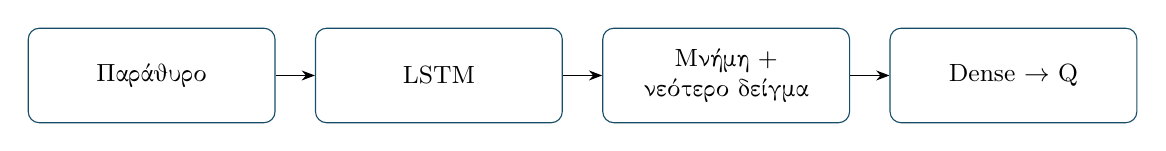
\begin{tikzpicture}[node distance=5mm,box/.style={draw=ink,rounded corners,align=center,font=\small,text width=29mm,minimum height=12mm},>=Stealth]
\node[box] (x) {Παράθυρο};\node[box,right=of x] (l) {LSTM};
\node[box,right=of l] (d) {Μνήμη +\\νεότερο δείγμα};\node[box,right=of d] (q) {Dense \ensuremath{\rightarrow} Q};
\draw[->] (x)--(l);\draw[->] (l)--(d);\draw[->] (d)--(q);
\end{tikzpicture}\end{center}

Ο διαχωρισμός βοηθά να ρωτήσουμε «έφταιξε η αρχιτεκτονική ή τα προηγούμενα βάρη;». Δεν αποδεικνύει μόνος του ποιο μοντέλο είναι καλύτερο. Οι παραλλαγές των αρχικών δημοσιεύσεων δεν ταυτίζονται αυτόματα με τα σημερινά διορθωμένα arms.
\src{\code{.lab/j64/final.json}: \code{research_contract}. \code{legacy/agent_lstm_fixed.py}, \code{legacy/networks_lstm.py}; \code{legacy/agent_lstm_v2.py}: \code{ARCHS['a1h']} = \code{l128-cat-d128-d128}. Παράθυρο δέκα ticks: \code{legacy/run_legacy.py}, \code{SEQ}.}

\page{9 · Transfer: ξεκινώ με εμπειρία}{Τι μεταφέρεται από έναν κόσμο σε άλλον;}
Στη μεταφορά μάθησης (transfer learning) εκπαιδεύουμε πρώτα σε περιβάλλον πηγής (source), κρατάμε τα βάρη και συνεχίζουμε στο περιβάλλον στόχου (target):
\[
 \theta_{\text{αρχή,target}}=\theta_{\text{τέλος,source}},\qquad
 \theta\leftarrow\theta-\eta\nabla_\theta L_{\rm target}(\theta).
\]
Το $L$ είναι το σφάλμα εκπαίδευσης, το $\nabla$ η κατεύθυνση μεταβολής του και το $\eta$ ο ρυθμός μάθησης. Ο Adam χρησιμοποιεί προσαρμοσμένη εκδοχή αυτής της ιδέας.

Για τον κύκλο 2 η πηγή είναι το \code{spike300_d5}, ενώ ο στόχος είναι το Poisson microservice περιβάλλον. Το LSTM+transfer μεταφέρει το fixed δίκτυο και το Dinos+Transfer V.2 το a1h.

\textbf{Πρακτικά:} το δίκτυο ίσως έχει ήδη μάθει ότι μια επίμονη άνοδος φορτίου απαιτεί έγκαιρη αντίδραση. Όμως τα ίδια βάρη μπορεί να είναι ακατάλληλα για τη νέα σχέση ουράς, κόστους και latency. Αυτό λέγεται αρνητική μεταφορά (negative transfer).

Στο σημερινό orig-family πρωτόκολλο αντιγράφονται τα βάρη σε καινούργιο online και target δίκτυο. Η replay μνήμη και ο optimizer αρχίζουν φρέσκοι. Συνεχίζουμε να εκπαιδεύουμε \textbf{όλο} το δίκτυο. Δεν είναι η μελλοντική QC4, όπου ο encoder παγώνει.

\idea{«Λιγότερα βήματα στο target» δεν σημαίνει λιγότερη συνολική εργασία. Χρεώνουμε source, target και αξιολόγηση.}
\think{Ένα μοντέλο χρειάζεται λιγότερα target ticks μετά από μεγάλη προεκπαίδευση. Αρκεί αυτό για ισχυρισμό οικονομίας;}
\src{\code{legacy/c5_protocol.py}: κλάδος \code{elif otr}, \code{mk_scratch}, \code{load_weights}. Ακριβής πηγή και χρεώσεις: \code{.lab/j64/final.json}, \code{research_contract}. Δεν υποθέτουμε ότι δύο διαφορετικές σημασίες χαρακτηριστικών γίνονται ίδιες επειδή έχουν ίδιο πλήθος θέσεων.}

\page{10 · DERP και HPA}{Άλλες αρχιτεκτονικές, άλλοι κανόνες}
Ο \textbf{DERP} χρησιμοποιεί MLP με δύο κρυφά επίπεδα πλάτους $128$ και έξοδο αξιών ενεργειών. Ο αρχικός βλέπει μόνο την τωρινή παρατήρηση. Ο \textbf{enhanced DERP} (\code{derp_hist10}) βλέπει δέκα διαδοχικές παρατηρήσεις απλωμένες σε ένα διάνυσμα. Έτσι έχει πρόσβαση σε ιστορικό χωρίς αναδρομική μνήμη.

Προσοχή στο όνομα: η κλάση του αρχικού λέγεται DDQNAgent, αλλά ο υπολογισμός στόχου είναι DQN με μέγιστο στο target και συγχρονισμό μετά από κάθε replay. Τα δύο DERP arms διατηρούν αυτή τη μηχανική· δεν τους αποδίδουμε τις διορθώσεις των fixed/a1h.

Ο οριζόντιος ελεγκτής pods (HPA) είναι κανόνας, όχι νευρωνικό δίκτυο. Ο αρχικός SimpleAgent αυξάνει αν CPU \emph{ή} μνήμη ξεπεράσει το όριο, αλλιώς μειώνει. Δεν έχει ενέργεια αναμονής. Η διεπαφή του αρχικού είναι έξι χαρακτηριστικών· ο κύκλος 2 χρειάζεται ρητό adapter για τα επτά.

Το \textbf{HPA-demand} μας υπολογίζει:
\[
 \widehat\lambda_t=\alpha A_t+(1-\alpha)\widehat\lambda_{t-1},\qquad
 n^*=\left\lceil\frac{\widehat\lambda_t}{\mu u}\right\rceil.
\]
Το $A_t$ είναι παρατηρημένες αφίξεις, $\widehat\lambda_t$ εξομαλυμένη εκτίμηση, $\alpha$ βάρος του νέου δείγματος και $u$ επιθυμητή αξιοποίηση. Η οροφή $\lceil\cdot\rceil$ στρογγυλεύει προς τα πάνω. Ο ελεγκτής κάνει ένα βήμα προς $n^*$ μετρώντας και εκκρεμή pods. Το $u$ επιλέγεται στο val.

Αυτό είναι δικό μας αιτιακό σημείο αναφοράς, όχι πλήρης αναπαραγωγή του Kubernetes HPA. Το oracle με πρόσβαση στο μελλοντικό φορτίο είναι βοηθητική ευρετική, όχι απόδειξη βέλτιστης απόδοσης.
\src{\code{legacy/network_dense.py}, \code{legacy/ddqnagent.py}, \code{legacy/c5_protocol.py} (\code{derp_history}), \code{legacy/simpleagent.py}, \code{pms_reference.py}: \code{make_policy}.}

\page{11 · DRe-SCale: μαθαίνω την πολιτική}{LSTM-PPO, actor και critic}
Στο Q-learning συγκρίνουμε αξίες ενεργειών. Στο PPO εκπαιδεύουμε άμεσα μια πολιτική $\pi_\theta(a\mid s)$: πιθανότητα να επιλέξει ενέργεια $a$ στο $s$. Ο actor δίνει την πολιτική, ο critic εκτιμά την αξία $V(s)$.

Η προσαρμογή DRe-SCale εδώ είναι \textbf{εγγενής υλοποίηση RecurrentPPO σε PyTorch}, όχι εκτέλεση της βιβλιοθήκης sb3\_contrib. Έχει ξεχωριστά LSTM actor/critic μεγέθους $256$ και δύο dense επίπεδα $64$ μονάδων ανά κλάδο. Διαβάζει την τρέχουσα παρατήρηση και κρατά μνήμη κατά την ακολουθία, με reset στην αρχή επεισοδίου.

Ο λόγος πιθανοτήτων $\rho_t$ και ο clipped στόχος είναι:
\[
 \rho_t=\frac{\pi_\theta(a_t\mid s_t)}{\pi_{\rm old}(a_t\mid s_t)},\quad
 L_{\rm clip}=\mathbb E\big[\min(\rho_t\widehat A_t,
 \operatorname{clip}(\rho_t,1-\varepsilon,1+\varepsilon)\widehat A_t)\big].
\]
Το $\widehat A_t$ είναι \textbf{πλεονέκτημα} (advantage): πόσο καλύτερη πήγε η ενέργεια από την εκτίμηση του critic. Το $\varepsilon$ περιορίζει το κίνητρο για υπερβολικές αλλαγές· δεν είναι το exploration $\epsilon$ του DQN και δεν αποτελεί αυστηρή εγγύηση ορίου στην πολιτική.

Το advantage εκτιμάται από σταθμισμένα διαδοχικά σφάλματα $\delta_t=r_t+\gamma V(s_{t+1})-V(s_t)$ με generalized advantage estimation (GAE). Το PPO μαθαίνει από πρόσφατα rollouts αντί να τραβά αυθαίρετα παλιές εμπειρίες replay. Εκπαιδεύει επίσης τον critic να προσεγγίζει τις επιστροφές.

Χρησιμοποιούμε τις κοινές ενέργειες, reward και traces μας. Η αξιολόγηση είναι greedy. Οι διαφορές padding και τυχαιότητας από τη βιβλιοθήκη δεν έχουν επιβεβαιωθεί με differential test· δεν αναπαράγουμε αποτελέσματα του δημοσιευμένου paper.
\src{\code{rppo.py}: \code{RecurrentAC}, \code{RPPO.update}, docstring. Προέλευση: DRe-SCale [Μ3]· PPO [Μ2]. Το συμβόλαιο εξαιρεί εδώ κοινό παράθυρο δέκα ticks: η μνήμη PPO είναι αναδρομική, όχι ίδιο fixed-window input.}

\page{12 · Train, val, test}{Τι είναι επεισόδιο και πότε επιτρέπεται να διαλέξουμε;}
Ένα \textbf{επεισόδιο} (episode) είναι μια συνεχής διαδρομή από reset μέχρι τέλος. Ένα \textbf{tick} είναι μία απόφαση μέσα της. Το training budget μπορεί να τελειώσει στη μέση επεισοδίου. Ένα \textbf{checkpoint} είναι αντίγραφο βαρών εκείνη τη στιγμή.

\textbf{Διδακτικό παράδειγμα.} Αν ένα επεισόδιο έχει $5000$ ticks, μπορούμε να αποθηκεύσουμε checkpoint στα $1000$ training ticks και κατόπιν να το αξιολογήσουμε σε \emph{ολόκληρα} νέα επεισόδια των $5000$ ticks. Το μικρό training checkpoint δεν κόβει την αξιολόγηση στη μέση.

\begin{center}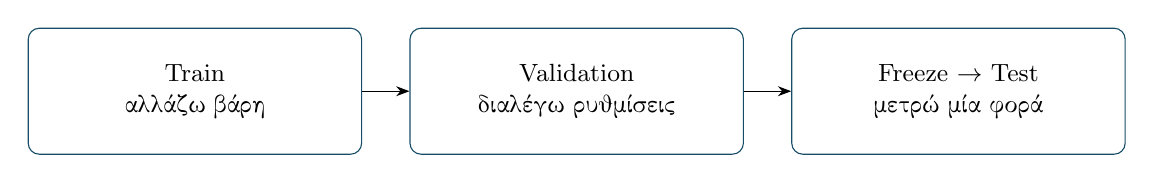
\begin{tikzpicture}[node distance=6mm,box/.style={draw=ink,rounded corners,align=center,font=\small,text width=40mm,minimum height=16mm},>=Stealth]
\node[box] (tr) {Train\\αλλάζω βάρη};\node[box,right=of tr] (v) {Validation\\διαλέγω ρυθμίσεις};\node[box,right=of v] (te) {Freeze \ensuremath{\rightarrow} Test\\μετρώ μία φορά};
\draw[->] (tr)--(v);\draw[->] (v)--(te);
\end{tikzpicture}\end{center}

Το \textbf{train} δίνει εμπειρίες για μάθηση. Το \textbf{validation (val)} επιλέγει ρυθμίσεις και checkpoint. Το \textbf{test} μένει κλειστό μέχρι να παγώσουν αυτές οι επιλογές. Αν επιστρέφουμε στο test για αλλαγές, το μετατρέπουμε σε νέο val και χάνουμε ανεξάρτητη επιβεβαίωση.

Ο training seed καθορίζει αρχικοποίηση και τυχαίες επιλογές μάθησης. Ο trace seed καθορίζει μια διαδρομή φορτίου. Πολλά traces του ίδιου εκπαιδευμένου δικτύου δεν ισοδυναμούν με πολλά ανεξάρτητα trainings.

Στο τωρινό περιβάλλον το επεισόδιο έχει προεπιλογή $5000$ ticks· το κύριο val έχει $20$ traces. Το test12 παραμένει κλειδωμένο στο harness που περιγράφουμε. Τα παλιά test10/test11 έχουν ήδη χρησιμοποιηθεί και δεν γίνονται ξανά ανεξάρτητα tests.
\think{Μπορεί μια καλή επίδοση στο val να χρησιμοποιηθεί για τελική δήλωση υπεροχής;}
\src{\code{poisson_ms.py}: \code{Params.ep_ticks}; \code{pms_adapter.py}: \code{SPLITS}, \code{LOCKED_SPLITS}. Προηγούμενες απορίες: \code{docs/tutorial.md}. Ιστορικά μήκη/ονόματα splits εκεί δεν αποτελούν νέο πρωτόκολλο.}

\page{13 · Πόσο σίγουροι είμαστε;}{Μέσος, IQM και διαστήματα αβεβαιότητας}
Κάθε εκπαίδευση μπορεί να δώσει άλλο αποτέλεσμα. Κρατάμε πίνακα αποτελεσμάτων $R_{ij}$: γραμμή $i$ = training seed, στήλη $j$ = κοινό test trace. Για σύγκριση δύο μοντέλων εξετάζουμε διαφορές στο ίδιο trace, όχι άσχετους εύκολους και δύσκολους κόσμους.

Ο μέσος χρησιμοποιεί όλες τις τιμές. Ο ενδοτεταρτημοριακός μέσος (interquartile mean, IQM) κρατά το μεσαίο μισό της ταξινομημένης κατανομής, με κατάλληλη διαχείριση ορίων όταν δεν χωρίζεται ακριβώς. Περιορίζει την επίδραση ακραίων τιμών, αλλά δεν εξαφανίζει τις αποτυχίες: τις αναφέρουμε επίσης.

\textbf{Διδακτικό παράδειγμα.} Για τις τέσσερις τιμές $(0,10,12,100)$, ο μέσος είναι $30.5$, ενώ ο IQM είναι $(10+12)/2=11$. Δεν αρκεί να δείξουμε έναν μόνο από αυτούς χωρίς την κατανομή.

Το bootstrap επαναδειγματοληπτεί από τα διαθέσιμα αποτελέσματα και επανυπολογίζει το στατιστικό. Ένα διάστημα εμπιστοσύνης (CI) εκτιμά την αβεβαιότητα από το πεπερασμένο δείγμα. Δεν σημαίνει ότι το επόμενο run θα πέσει εκεί με την ίδια πιθανότητα.

Εδώ χρειάζεται προσοχή στη δομή: κρατάμε χωριστά training seeds και κοινά traces, διατηρούμε το pairing και επαναδειγματοληπτούμε στο κατάλληλο επίπεδο. Δεν βαφτίζουμε κάθε tick ανεξάρτητο πείραμα. Το ακριβές σχέδιο bootstrap και οι υποθέσεις παγώνουν πριν την τελική ανάλυση.

\idea{Μικρό CI δεν διορθώνει κακό simulator, test leakage ή άνισο tuning budget.}
Η ανταμοιβή διαβάζεται μαζί με SLO, p95, pod-time, απορρίψεις και churn. Οι προκαθορισμένες υποθέσεις προστατεύουν από το να επιλέξουμε εκ των υστέρων μόνο τη σύγκριση που «πέτυχε».
\src{Απαιτήσεις κύκλου 2: \code{docs/cycle2_plan.md}, §4–6. Θεωρία αξιόπιστης RL αξιολόγησης: [Μ5, σ. 20]. Οι αριθμοί IQM είναι διδακτική αριθμητική, όχι αποτελέσματα του lab.}

\page{14 · Το κβαντικό δομικό υλικό}{Κατάσταση, περιστροφή, συσχέτιση, μέτρηση}
Ένα qubit περιγράφεται ως $\ket\psi=\alpha\ket0+\beta\ket1$, με $|\alpha|^2+|\beta|^2=1$. Τα $\alpha,\beta$ είναι μιγαδικά πλάτη· η μέτρηση δίνει $0$ ή $1$ με τις αντίστοιχες πιθανότητες. Δεν διαβάζουμε ταυτόχρονα όλες τις πιθανές απαντήσεις.

Μια περιστροφή $R_y(x)$ μπορεί να κωδικοποιήσει ένα κανονικοποιημένο χαρακτηριστικό ως γωνία:
\[
 R_y(x)\ket0=\cos(x/2)\ket0+\sin(x/2)\ket1.
\]
Το $x$ είναι γωνία σε ακτίνια, όχι ακατέργαστη CPU. Χρειάζεται κοινή, σαφής προεπεξεργασία. Μια πύλη σύζευξης μπορεί να δημιουργήσει διεμπλοκή (entanglement), δηλαδή κατάσταση πολλών qubits που δεν γράφεται ως ανεξάρτητα επιμέρους qubits. Αυτό δεν εγγυάται χρήσιμη μάθηση.

Ένα παραμετρικό κβαντικό κύκλωμα (PQC), που βελτιστοποιείται μεταβολικά (VQC), δίνει μετρήσιμα χαρακτηριστικά:
\[
 z_j(x,\theta)=\langle\psi(x,\theta)|Z_j|\psi(x,\theta)\rangle.
\]
Το $\theta$ είναι γωνίες που μαθαίνουμε και το $Z_j$ παρατηρήσιμο στο qubit $j$. Το $z_j$ είναι μέση μέτρηση μεταξύ $-1$ και $1$. Το $Z$ δίνει $+1$ για αποτέλεσμα $0$ και $-1$ για $1$. Διδακτικά, $75\%$ μηδενικά δίνουν μέση τιμή $0.5$. Μια κλασική έξοδος $Q_a=b_a+\sum_j w_{aj}z_j$ μετατρέπει αυτές τις τιμές σε αξίες ενεργειών· τα $w,b$ επίσης μετράνε ως παράμετροι.

\idea{Το κύκλωμα είναι ένας εκπαιδεύσιμος μετασχηματισμός χαρακτηριστικών. Η αξία του ελέγχεται από τις αποφάσεις autoscaling που βελτιώνει.}
\src{Βασική κωδικοποίηση και data re-uploading: [Κ1, σ. 20]. Ερμηνεία προσδοκώμενης τιμής και gradients: [Κ2]. Οι εξισώσεις δείχνουν πιθανό σχεδιασμό, όχι ήδη μετρημένο κβαντικό μοντέλο του lab.}

\page{15 · QC1 και QC4}{Οι δύο προτάσεις για το πρώτο screening}
\textbf{QC1 — παράθυρο \ensuremath{\rightarrow} κύκλωμα \ensuremath{\rightarrow} αξίες ενεργειών.} Αντί για LSTM/MLP, ένα κύκλωμα επεξεργάζεται το παράθυρο. Με επαναφόρτωση δεδομένων (data re-uploading) παρεμβάλλουμε νέες εισόδους ανάμεσα σε εκπαιδεύσιμους μετασχηματισμούς:
\[
 \ket{\psi_L}=U_{\theta_L}E(x_L)\cdots U_{\theta_1}E(x_1)\ket0.
\]
Το $E$ κωδικοποιεί δεδομένα και το $U$ είναι μετασχηματισμός με παραμέτρους. Οι δεξιότερες πράξεις γίνονται πρώτες. Τα $x_1,\ldots,x_L$ μπορούν να είναι διαδοχικά χρονικά δείγματα. Στο τέλος μετράμε και παράγουμε Q για τις ενέργειες.

\emph{Σημασία για το Redis:} η πρόσφατη άνοδος αφίξεων αλλάζει την κβαντική κατάσταση, όπως η είσοδος αλλάζει τα κρυφά χαρακτηριστικά ενός κλασικού δικτύου. Η επαναφόρτωση αυξάνει την εκφραστικότητα· δεν είναι αυτομάτως LSTM ούτε απεριόριστη μνήμη. Ο έλεγχος γίνεται απέναντι σε μικρό κλασικό μοντέλο με αντιστοιχισμένο αριθμό παραμέτρων.

\textbf{QC4 — encoder \ensuremath{\rightarrow} κβαντική κεφαλή \ensuremath{\rightarrow} αξίες ενεργειών.} Ένας κλασικός encoder (συμπιεστής παρατηρήσεων σε χρήσιμα χαρακτηριστικά) $f_\phi$ προεκπαιδεύεται στο source και μετά δεν αλλάζει:
\[
 h=f_{\phi_{\rm frozen}}(s),\qquad Q(s,a)=g_\theta(h)_a.
\]
Η κεφαλή $g_\theta$ περιέχει μικρό VQC και εκπαιδεύεται στο target. «Παγωμένο» σημαίνει μηδενικές ενημερώσεις στα βάρη $\phi$, όχι δωρεάν εκτέλεση του encoder.

\emph{Σημασία:} ίσως χρειάζεται να μεταφέρουμε/προσαρμόσουμε λίγες μόνο παραμέτρους όταν αλλάζει το περιβάλλον. Ο κρίσιμος έλεγχος είναι \textbf{ο ίδιος παγωμένος encoder με κλασική κεφαλή ίσων trainable παραμέτρων}. Κρατάμε και το συνολικό μέγεθος του συστήματος· δεν εξαφανίζουμε τον encoder από τη λογιστική.
\src{\code{docs/PLAN.md}, §8.3–8.5· \code{docs/rules/paused.md}, D5. QC1 και QC4 έχουν αποφασιστεί ως screening και παραμένουν σε παύση. Θεωρία re-uploading: [Κ1].}

\page{16 · QC2, QC3 και QC5}{Τρεις διαφορετικές θέσεις για ένα κύκλωμα}
\textbf{QC2 — ιστορικό \ensuremath{\rightarrow} κβαντικές πύλες LSTM \ensuremath{\rightarrow} μνήμη/Q.} Οι πύλες της σ. 7 θα παράγονται από κβαντικά χαρακτηριστικά, π.χ. $f_t=\sigma(Az_\theta([x_t,h_{t-1}])+b)$. Το $z_\theta$ είναι διάνυσμα μετρήσεων και τα $A,b$ κλασική προσαρμογή διαστάσεων.

Η αναδρομική μνήμη συνεχίζει να ενημερώνεται αριθμητικά. Δεν σημαίνει ότι κρατάμε ένα qubit σε συνεχή λειτουργία επί ολόκληρο επεισόδιο. Χρειάζονται πολλά κυκλώματα ανά παράθυρο και πύλη· μικρότερος αριθμός παραμέτρων δεν εγγυάται μικρότερο χρόνο.

\textbf{QC3 — μικρός GRU \ensuremath{\rightarrow} κβαντική κεφαλή \ensuremath{\rightarrow} Q.} Το gated recurrent unit (GRU) συμπυκνώνει το ιστορικό με πύλες ενημέρωσης/επαναφοράς και μία κρυφή κατάσταση, αντί για ξεχωριστή cell memory LSTM. Σε τυπική σύμβαση:
\[
 h_t=(1-z_t)\odot\widetilde h_t+z_t\odot h_{t-1}.
\]
Το $z_t$ είναι πύλη διατήρησης και το $\widetilde h_t$ υποψήφια νέα μνήμη. Εδώ το $z_t$ δεν είναι η μέτρηση της σ. 14. Η κεφαλή μετατρέπει το συμπιεσμένο ιστορικό σε Q. Χρειαζόμαστε ίδιο μικρό encoder με κλασική κεφαλή: η οικονομία μπορεί να προέρχεται από τη συρρίκνωση του encoder.

\textbf{QC5 — ιστορικό \ensuremath{\rightarrow} σταθερό κύκλωμα \ensuremath{\rightarrow} πρόβλεψη φορτίου.} Ένα σταθερό τυχαίο κύκλωμα παράγει χαρακτηριστικά $z_t$ ιστορικού· εκπαιδεύεται μόνο γραμμική έξοδος πρόβλεψης. Με πίνακα χαρακτηριστικών $Z$ και μελλοντικών φορτίων $y$:
\[
 w=(Z^\top Z+\alpha I)^{-1}Z^\top y.
\]
Αυτή είναι ridge regression: το $\alpha>0$ περιορίζει μεγάλα βάρη, το $I$ είναι μοναδιαίος πίνακας. Η πρόβλεψη προστίθεται στην κατάσταση του ελεγκτή. Η ακριβής χρονική μνήμη του reservoir μένει να οριστεί πριν από πείραμα. Σύγκριση με κλασικό echo-state reservoir και ίδια ιστορικά δεδομένα, χωρίς διαρροή μελλοντικού φορτίου.
\src{\code{docs/PLAN.md}, §8.4: QC2/QC3/QC5 είναι εναλλακτικές προτάσεις, όχι αποτελέσματα. GRU: PyTorch [Μ4]. Οι εξισώσεις είναι επεξηγηματικά πρότυπα, όχι παγωμένη προδιαγραφή υλοποίησης.}

\page{17 · QC6 και QC7}{Ομοιότητα παραθύρων και προσοχή}
\textbf{QC6 — παράθυρα \ensuremath{\rightarrow} ομοιότητες \ensuremath{\rightarrow} καθεστώς φορτίου.} Θέλουμε να ξεχωρίσουμε ήρεμο φορτίο, άνοδο και έκρηξη. Ένα παράθυρο κωδικοποιείται σε κανονικοποιημένη κατάσταση $\ket{\psi(x)}$. Για δύο παράθυρα, ο swap test εκτιμά την ομοιότητα:
\[
 \Pr(\text{βοηθητικό qubit}=0)
 =\frac{1+|\langle\psi(x)|\psi(y)\rangle|^2}{2}.
\]
Το εσωτερικό γινόμενο μετρά επικάλυψη κβαντικών καταστάσεων. Η ομοιότητα αφορά την \emph{επιλεγμένη κωδικοποίηση}, όχι αναγκαστικά ό,τι θεωρούμε χρήσιμο στο autoscaling.

Με ομαδοποίηση (clustering) παρόμοιων παραθύρων, η ετικέτα καθεστώτος μπορεί να γίνει πρόσθετο χαρακτηριστικό ή να επιλέγει πολιτική από βιβλιοθήκη. Το quantum k-means ακολουθεί την ιδέα «ανάθεση στην κοντινότερη ομάδα, ενημέρωση κέντρων», με κβαντικό υπολογισμό ομοιότητας σε προτεινόμενη εκδοχή του. Η φόρτωση δεδομένων, τα κέντρα και ο τρόπος ενημέρωσης χρειάζονται συγκεκριμένο σχέδιο. Έλεγχος: κλασικό clustering/ίδια χαρακτηριστικά και ίδιο tuning.

\textbf{QC7 — ομοιότητες \ensuremath{\rightarrow} βάρη attention \ensuremath{\rightarrow} χρονικά χαρακτηριστικά.} Η προσοχή δίνει μεγαλύτερο βάρος στα χρήσιμα παλιά δείγματα. Ένα επεξηγηματικό σχήμα είναι:
\[
 K_{ij}=|\langle\psi(x_i)|\psi(x_j)\rangle|^2,\quad
 a_{ij}=\frac{e^{\beta K_{ij}}}{\sum_k e^{\beta K_{ik}}},\quad
 h_i=\sum_j a_{ij}v_j.
\]
Τα $v_j$ είναι χαρακτηριστικά προς συνδυασμό και το $\beta$ ελέγχει πόσο έντονα προτιμώνται μεγάλες ομοιότητες. Αυτό είναι \textbf{διδακτική πιθανή κατασκευή}, όχι συμφωνημένο attention μοντέλο. Στο autoscaling επιτρέπονται μόνο παρελθοντικά/τωρινά δείγματα.

Για παράθυρο μήκους $k$, όλα τα ζεύγη χρειάζονται τάξη $k^2$ συγκρίσεων. Μπορεί να κοστίζουν περισσότερο από όσο ωφελούν. Το QC7 παραμένει πιο μακρινή πρόταση.
\src{\code{docs/PLAN.md}, §8.4: QC6/QC7, σύνδεση QuantuML. Swap test: [Κ3, σ. 20]. Η εξίσωση χρησιμοποιεί καθαρές καταστάσεις και ιδανικό κύκλωμα.}

\page{18 · Πώς μαθαίνει και τι δεν αποδεικνύει}{Κβαντικό αποτέλεσμα χρειάζεται κλασικό έλεγχο}
Οι κλασικοί optimizers μπορούν να αλλάζουν τις γωνίες του κυκλώματος από gradients. Για μία κατάλληλη πύλη περιστροφής Pauli, όταν η παράμετρος εμφανίζεται με τη συνήθη μορφή, ο κανόνας μετατόπισης παραμέτρου (parameter shift) δίνει:
\[
 \frac{\partial f}{\partial\theta}
 =\frac{f(\theta+\pi/2)-f(\theta-\pi/2)}{2}.
\]
Το $f$ είναι προσδοκώμενη μέτρηση. Δεν είναι καθολικός τύπος για κάθε πύλη ή κοινή παράμετρο σε πολλές θέσεις. Σε simulator μπορεί να χρησιμοποιηθεί και adjoint differentiation, με διαφορετικό υπολογιστικό κόστος.

Στο πραγματικό κύκλωμα εκτελούμε επαναλήψεις μέτρησης (shots). Για μέτρηση $Z$ με αποτελέσματα $\pm1$, η μέση τιμή έχει τυπικό σφάλμα $\sqrt{(1-z^2)/M}$ μετά από $M$ ανεξάρτητα ιδανικά shots. Θόρυβος συσκευής μπορεί να προσθέσει και μεροληψία, όχι μόνο διακύμανση.

\textbf{Τι μετράμε σε μια δίκαιη σύγκριση;} Ποιότητα αποφάσεων, SLO, συνολικές/trainable παράμετροι, μέγεθος checkpoint, κόστος φόρτωσης/encoder/κεφαλής, πλήθος κυκλωμάτων και shots, χρόνος απόφασης και προεκπαίδευση. Αντικατάσταση μικρής κεφαλής δεν μικραίνει μαγικά έναν μεγάλο encoder.

\textbf{Τι δεν ισχυριζόμαστε;} Χρόνος σε κλασικό simulator δεν αποδεικνύει κβαντικό speed-up. Λιγότερες παράμετροι χρειάζονται parameter-matched κλασικό έλεγχο· ίσο πλήθος δεν εγγυάται ίση εκφραστικότητα. Εκθετικά πολλές συνιστώσες κατάστασης δεν σημαίνουν εκθετικά πολλές προσβάσιμες απαντήσεις.

Η παλιά «Quantum» παραλλαγή του αρχικού κώδικα χρησιμοποιεί κύκλωμα μόνο για τυχαία εξερεύνηση· δεν εκπαιδεύει κβαντική Q-function. Δεν είναι τα QC1–QC7. Τα screens και η IBM εκτέλεση παραμένουν σε παύση· καμία εξήγηση εδώ δεν αποτελεί άδεια εκτέλεσης.
\src{Gradient: [Κ2]. Περιορισμοί/αρχική παραλλαγή: \code{docs/PLAN.md}, F4, §8.3–8.8· \code{docs/rules/paused.md}. Το shot error προκύπτει από τη διακύμανση ανεξάρτητων μεταβλητών $\pm1$.}

\page{19 · Έλεγχος κατανόησης}{Κλείσε το PDF πριν κοιτάξεις τις απαντήσεις}
\textbf{1. Γιατί να αυξήσουμε pods πριν ανέβει πολύ η CPU;}\\
Επειδή το νέο pod χρειάζεται χρόνο εκκίνησης. Η τάση φορτίου και η ουρά ίσως προειδοποιούν νωρίτερα. Δεν αποδεικνύεται από αυτό ότι κάθε πρόωρη αύξηση είναι καλή.

\textbf{2. Τι κερδίζουμε με κοινά traces;}\\
Τα μοντέλα αντιμετωπίζουν την ίδια εξωτερική δυσκολία. Οι διαφορές δεν οφείλονται στο ότι το ένα έτυχε να δει πιο ήρεμο φορτίο. Χρειαζόμαστε επιπλέον πολλούς training seeds.

\textbf{3. Γιατί το Q μπορεί να προτιμά προσωρινό κόστος;}\\
Εκτιμά και μελλοντικές ανταμοιβές. Η αύξηση τώρα μπορεί να αποτρέψει μεγαλύτερη ουρά, παραβιάσεις και απορρίψεις αργότερα.

\textbf{4. Τι προσφέρει το LSTM σε ίδια τελευταία μέτρηση;}\\
Μπορεί να συμπυκνώνει διαφορετικές χρονικές τάσεις. Δεν εγγυάται ότι έμαθε τη σωστή σχέση· αυτό ελέγχεται σε ανεξάρτητη αξιολόγηση.

\textbf{5. Λιγότερη εκπαίδευση στο target αρκεί;}\\
Όχι για συνολική οικονομία. Συνυπολογίζουμε source, fine-tuning, tuning και inference. Αναφέρουμε χωριστά την ταχύτητα προσαρμογής.

\textbf{6. Μπορώ να δηλώσω νίκη από το val;}\\
Το val υποστηρίζει επιλογή. Η τελική επιβεβαίωση γίνεται αφού παγώσουν οι επιλογές, στο κλειστό test με προδηλωμένη ανάλυση.

\textbf{7. Ποιος έλεγχος ξεχωρίζει την QC4 από απλό πάγωμα;}\\
Ίδιος frozen encoder και κλασική κεφαλή με αντιστοιχισμένες trainable παραμέτρους. Αλλιώς το όφελος ίσως προέρχεται μόνο από το πάγωμα.

\textbf{8. Αν το κύκλωμα έχει λιγότερα βάρη, είναι ταχύτερο;}\\
Όχι απαραίτητα. Κυκλώματα, shots, gradients, φόρτωση και επικοινωνία μπορεί να κυριαρχούν. Χρειάζεται κατάλληλη μέτρηση· simulator timing δεν αποδεικνύει κβαντικό speed-up.
\src{Ερωτήσεις βασισμένες στις σ. 2–18. Παιδαγωγική επιλογή: worked examples και ανάκληση, \code{docs/tutorials/PLAYBOOK.md}. Ο έλεγχος από agent είναι εκδοτικός έλεγχος, όχι μελέτη κατανόησης ανθρώπων.}

\page{20 · Πηγές και χάρτης ελέγχου}{Για να ελέγξεις ή να συνεχίσεις το διάβασμα}
{\small
\textbf{Πιθανότητες}\par
[Π1] Pishro-Nik, \emph{Introduction to Probability, Statistics, and Random Processes}, \href{https://www.probabilitycourse.com/chapter11/11_1_2_basic_concepts_of_the_poisson_process.php}{§11.1.2: Poisson process}.\par
[Π2] Ίδιο βιβλίο, \href{https://www.probabilitycourse.com/chapter11/11_1_4_nonhomogeneous_poisson_processes.php}{§11.1.4: Nonhomogeneous Poisson processes}.

\textbf{Μάθηση}\par
[Μ1] van Hasselt, Guez, Silver, \href{https://arxiv.org/abs/1509.06461}{Deep Reinforcement Learning with Double Q-learning}.\par
[Μ2] Schulman et al., \href{https://arxiv.org/abs/1707.06347}{Proximal Policy Optimization Algorithms}.\par
[Μ3] Agarwal, Rodriguez, Buyya, DRe-SCale, \href{https://doi.org/10.1109/TSC.2024.3387661}{IEEE TSC, DOI 10.1109/TSC.2024.3387661}. \href{https://github.com/SidAg26/DRe-SCale}{Αρχικός κώδικας}. Δική μας προσαρμογή: \code{rppo.py}.\par
[Μ4] PyTorch, \href{https://docs.pytorch.org/docs/stable/generated/torch.nn.LSTM.html}{LSTM} και \href{https://docs.pytorch.org/docs/stable/generated/torch.nn.GRU.html}{GRU}: ακριβείς εξισώσεις πυλών.\par
[Μ5] Agarwal et al., \href{https://arxiv.org/abs/2108.13264}{Deep RL at the Edge of the Statistical Precipice}: IQM και αβεβαιότητα. Το σχέδιο επαναδειγματοληψίας εξαρτάται από το δικό μας πείραμα.

\textbf{Κβαντική μάθηση}\par
[Κ1] PennyLane, \href{https://pennylane.ai/demos/tutorial_data_reuploading_classifier}{Data-reuploading classifier}.\par
[Κ2] PennyLane, \href{https://docs.pennylane.ai/en/stable/code/api/pennylane.gradients.param_shift.html}{Parameter-shift gradients}.\par
[Κ3] Buhrman et al., \href{https://arxiv.org/abs/quant-ph/0102001}{Quantum Fingerprinting}: δοκιμή επικάλυψης (swap test).

\textbf{Ποια έκδοση περιγράφεται}\par
Ανάγνωση κώδικα: \code{code-poisson} HEAD \code{cc83534}; frozen environment \code{238003f}, frozen harness \code{b609b93}. Ιστορική διασταύρωση: \code{code-tuning} \code{5eae972} και read-only αρχικός κώδικας \code{~/simulations/redisk8s/timeseries/Pytorch/}.\par
Τα σύντομα paths στις σελίδες είναι σχετικά με \code{code-poisson/tuning/}. Αντιστοίχιση ονομάτων/arms: \code{.lab/j64/final.json}, \code{research_contract}. Τα προτεινόμενα μελλοντικά budgets δεν αποτελούν τελική εγκεκριμένη εκτέλεση.\par
Κβαντικά σχέδια: \code{docs/PLAN.md}, §8.4. Η τωρινή προτεραιότητα και η παύση υπερισχύουν παλιών σχεδίων: \code{docs/STATE.md}, \code{docs/rules/paused.md}.\par
Πρακτικές διδασκαλίας, συνέχεια επόμενων tutorials και ανεξάρτητοι έλεγχοι: \code{docs/tutorials/PLAYBOOK.md}, \code{docs/tutorials/REVIEW.md}. Πρόσβαση στις online πηγές: 29/10/2026.
}
\end{document}
